\documentclass{standalone}
\usepackage{tikz}
\usetikzlibrary{patterns, positioning}


\begin{document}
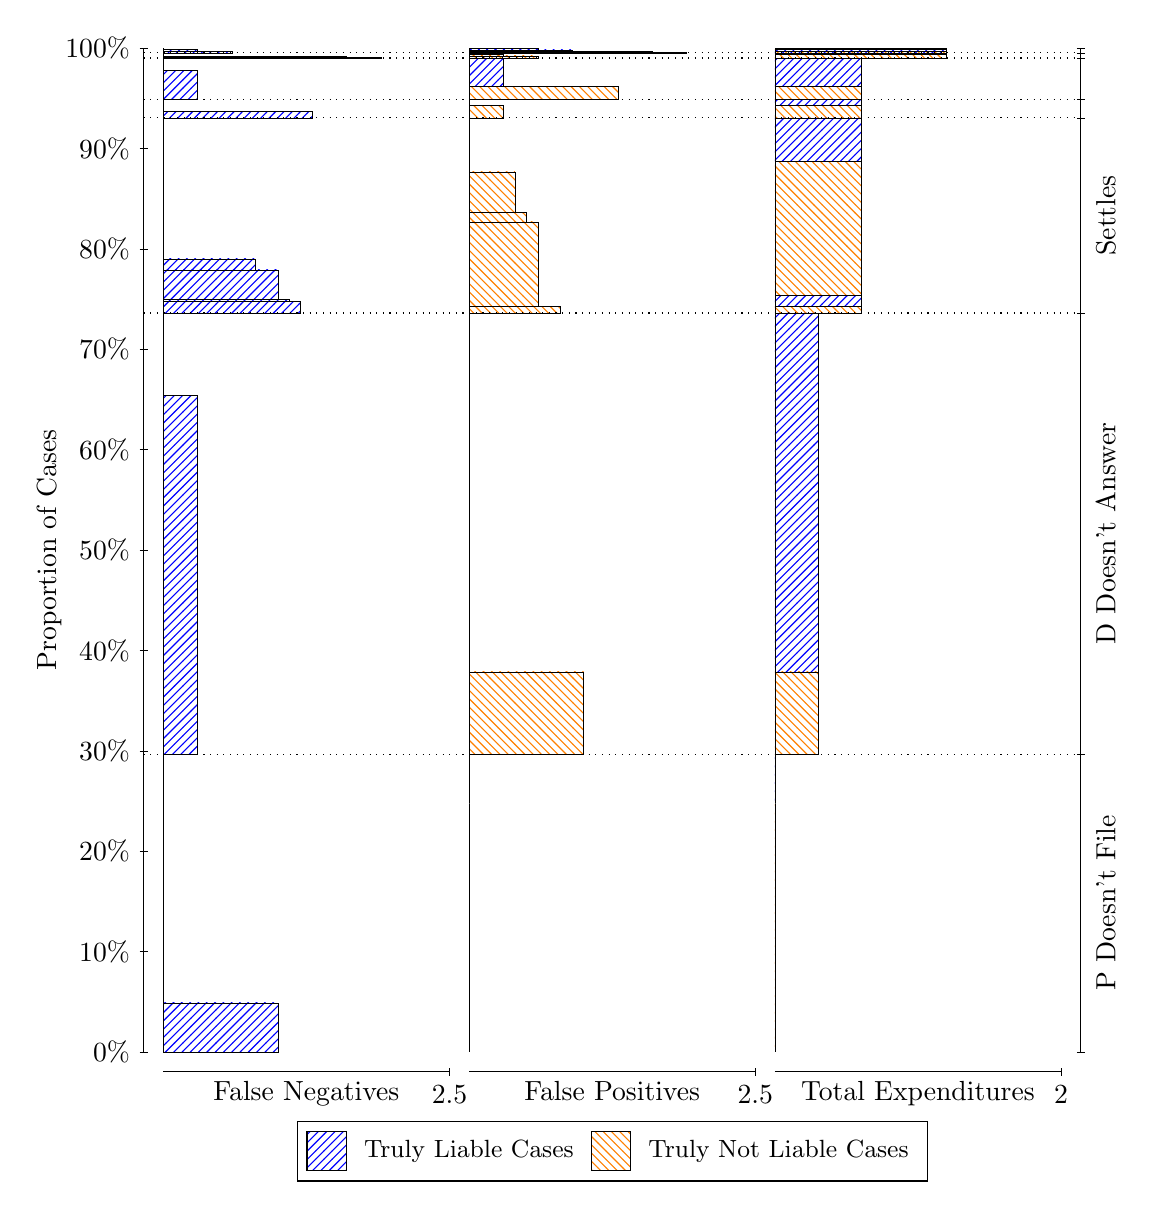
\begin{tikzpicture}
\draw[black, very thin] (1.5,1.75) -- (1.5,14.5);
\node[rotate=90, text=black, anchor=center] at (0.3, 8.125) {Proportion of Cases};
\draw[black, very thin] (1.45,1.75) -- (1.55,1.75);
\node[text=black, anchor=east] at (1.45, 1.75) {0\%};
\draw[black, very thin] (1.45,3.025) -- (1.55,3.025);
\node[text=black, anchor=east] at (1.45, 3.025) {10\%};
\draw[black, very thin] (1.45,4.3) -- (1.55,4.3);
\node[text=black, anchor=east] at (1.45, 4.3) {20\%};
\draw[black, very thin] (1.45,5.575) -- (1.55,5.575);
\node[text=black, anchor=east] at (1.45, 5.575) {30\%};
\draw[black, very thin] (1.45,6.85) -- (1.55,6.85);
\node[text=black, anchor=east] at (1.45, 6.85) {40\%};
\draw[black, very thin] (1.45,8.125) -- (1.55,8.125);
\node[text=black, anchor=east] at (1.45, 8.125) {50\%};
\draw[black, very thin] (1.45,9.4) -- (1.55,9.4);
\node[text=black, anchor=east] at (1.45, 9.4) {60\%};
\draw[black, very thin] (1.45,10.675) -- (1.55,10.675);
\node[text=black, anchor=east] at (1.45, 10.675) {70\%};
\draw[black, very thin] (1.45,11.95) -- (1.55,11.95);
\node[text=black, anchor=east] at (1.45, 11.95) {80\%};
\draw[black, very thin] (1.45,13.225) -- (1.55,13.225);
\node[text=black, anchor=east] at (1.45, 13.225) {90\%};
\draw[black, very thin] (1.45,14.5) -- (1.55,14.5);
\node[text=black, anchor=east] at (1.45, 14.5) {100\%};

\draw[black, very thin] (13.4,1.75) -- (13.4,14.5);
\draw[black, very thin] (13.35,1.75) -- (13.45,1.75);
\node[anchor=west] at (13.35, 1.75) {};
\draw[black, very thin] (13.35,5.5323) -- (13.45,5.5323);
\node[anchor=west] at (13.35, 5.5323) {};
\draw[black, very thin] (13.35,11.135) -- (13.45,11.135);
\node[anchor=west] at (13.35, 11.135) {};
\draw[black, very thin] (13.35,13.613) -- (13.45,13.613);
\node[anchor=west] at (13.35, 13.613) {};
\draw[black, very thin] (13.35,13.85) -- (13.45,13.85);
\node[anchor=west] at (13.35, 13.85) {};
\draw[black, very thin] (13.35,14.373) -- (13.45,14.373);
\node[anchor=west] at (13.35, 14.373) {};
\draw[black, very thin] (13.35,14.438) -- (13.45,14.438);
\node[anchor=west] at (13.35, 14.438) {};
\draw[black, very thin] (13.35,14.5) -- (13.45,14.5);
\node[anchor=west] at (13.35, 14.5) {};

\draw[black, very thin, pattern color=blue, pattern=north east lines] (1.75,1.75) rectangle (3.2033,2.3746);
\draw[black, very thin, pattern color=orange, pattern=north west lines] (1.75,2.3746) rectangle (1.75,5.5323);
\draw[black, very thin, pattern color=blue, pattern=north east lines] (1.75,5.5323) rectangle (2.186,10.09);
\draw[black, very thin, pattern color=orange, pattern=north west lines] (1.75,10.09) rectangle (1.75,11.135);
\draw[black, very thin, pattern color=blue, pattern=north east lines] (1.75,11.135) rectangle (3.494,11.282);
\draw[black, very thin, pattern color=blue, pattern=north east lines] (1.75,11.282) rectangle (3.3487,11.308);
\draw[black, very thin, pattern color=blue, pattern=north east lines] (1.75,11.308) rectangle (3.2033,11.683);
\draw[black, very thin, pattern color=blue, pattern=north east lines] (1.75,11.683) rectangle (2.9127,11.821);
\draw[black, very thin, pattern color=orange, pattern=north west lines] (1.75,11.821) rectangle (1.75,13.613);
\draw[black, very thin, pattern color=blue, pattern=north east lines] (1.75,13.613) rectangle (3.6393,13.696);
\draw[black, very thin, pattern color=orange, pattern=north west lines] (1.75,13.696) rectangle (1.75,13.85);
\draw[black, very thin, pattern color=blue, pattern=north east lines] (1.75,13.85) rectangle (2.186,14.212);
\draw[black, very thin, pattern color=orange, pattern=north west lines] (1.75,14.212) rectangle (1.75,14.373);
\draw[black, very thin, pattern color=blue, pattern=north east lines] (1.75,14.373) rectangle (4.5113,14.378);
\draw[black, very thin, pattern color=blue, pattern=north east lines] (1.75,14.378) rectangle (4.0753,14.394);
\draw[black, very thin, pattern color=orange, pattern=north west lines] (1.75,14.394) rectangle (1.75,14.438);
\draw[black, very thin, pattern color=blue, pattern=north east lines] (1.75,14.438) rectangle (2.622,14.462);
\draw[black, very thin, pattern color=blue, pattern=north east lines] (1.75,14.462) rectangle (2.186,14.478);
\draw[black, very thin, pattern color=orange, pattern=north west lines] (1.75,14.478) rectangle (1.75,14.5);
\draw[black, very thin, pattern color=orange, pattern=north west lines] (5.6333,1.75) rectangle (5.6333,4.9077);
\draw[black, very thin, pattern color=blue, pattern=north east lines] (5.6333,4.9077) rectangle (5.6333,5.5323);
\draw[black, very thin, pattern color=orange, pattern=north west lines] (5.6333,5.5323) rectangle (7.0867,6.5778);
\draw[black, very thin, pattern color=blue, pattern=north east lines] (5.6333,6.5778) rectangle (5.6333,11.135);
\draw[black, very thin, pattern color=orange, pattern=north west lines] (5.6333,11.135) rectangle (6.796,11.215);
\draw[black, very thin, pattern color=orange, pattern=north west lines] (5.6333,11.215) rectangle (6.5053,12.291);
\draw[black, very thin, pattern color=orange, pattern=north west lines] (5.6333,12.291) rectangle (6.36,12.414);
\draw[black, very thin, pattern color=orange, pattern=north west lines] (5.6333,12.414) rectangle (6.2147,12.927);
\draw[black, very thin, pattern color=blue, pattern=north east lines] (5.6333,12.927) rectangle (5.6333,13.613);
\draw[black, very thin, pattern color=orange, pattern=north west lines] (5.6333,13.613) rectangle (6.0693,13.767);
\draw[black, very thin, pattern color=blue, pattern=north east lines] (5.6333,13.767) rectangle (5.6333,13.85);
\draw[black, very thin, pattern color=orange, pattern=north west lines] (5.6333,13.85) rectangle (7.5227,14.011);
\draw[black, very thin, pattern color=blue, pattern=north east lines] (5.6333,14.011) rectangle (6.0693,14.373);
\draw[black, very thin, pattern color=orange, pattern=north west lines] (5.6333,14.373) rectangle (6.5053,14.399);
\draw[black, very thin, pattern color=orange, pattern=north west lines] (5.6333,14.399) rectangle (6.0693,14.417);
\draw[black, very thin, pattern color=blue, pattern=north east lines] (5.6333,14.417) rectangle (5.6333,14.438);
\draw[black, very thin, pattern color=orange, pattern=north west lines] (5.6333,14.438) rectangle (8.3947,14.443);
\draw[black, very thin, pattern color=orange, pattern=north west lines] (5.6333,14.443) rectangle (7.9587,14.46);
\draw[black, very thin, pattern color=blue, pattern=north east lines] (5.6333,14.46) rectangle (6.9413,14.476);
\draw[black, very thin, pattern color=blue, pattern=north east lines] (5.6333,14.476) rectangle (6.5053,14.5);
\draw[black, very thin, pattern color=orange, pattern=north west lines] (9.5167,1.75) rectangle (9.5167,4.9077);
\draw[black, very thin, pattern color=blue, pattern=north east lines] (9.5167,4.9077) rectangle (9.5167,5.5323);
\draw[black, very thin, pattern color=orange, pattern=north west lines] (9.5167,5.5323) rectangle (10.062,6.5778);
\draw[black, very thin, pattern color=blue, pattern=north east lines] (9.5167,6.5778) rectangle (10.062,11.135);
\draw[black, very thin, pattern color=orange, pattern=north west lines] (9.5167,11.135) rectangle (10.607,11.215);
\draw[black, very thin, pattern color=blue, pattern=north east lines] (9.5167,11.215) rectangle (10.607,11.354);
\draw[black, very thin, pattern color=orange, pattern=north west lines] (9.5167,11.354) rectangle (10.607,13.065);
\draw[black, very thin, pattern color=blue, pattern=north east lines] (9.5167,13.065) rectangle (10.607,13.613);
\draw[black, very thin, pattern color=orange, pattern=north west lines] (9.5167,13.613) rectangle (10.607,13.767);
\draw[black, very thin, pattern color=blue, pattern=north east lines] (9.5167,13.767) rectangle (10.607,13.85);
\draw[black, very thin, pattern color=orange, pattern=north west lines] (9.5167,13.85) rectangle (10.607,14.011);
\draw[black, very thin, pattern color=blue, pattern=north east lines] (9.5167,14.011) rectangle (10.607,14.373);
\draw[black, very thin, pattern color=orange, pattern=north west lines] (9.5167,14.373) rectangle (11.697,14.417);
\draw[black, very thin, pattern color=blue, pattern=north east lines] (9.5167,14.417) rectangle (11.697,14.438);
\draw[black, very thin, pattern color=orange, pattern=north west lines] (9.5167,14.438) rectangle (11.697,14.455);
\draw[black, very thin, pattern color=blue, pattern=north east lines] (9.5167,14.455) rectangle (11.697,14.479);
\draw[black, very thin, pattern color=orange, pattern=north west lines] (9.5167,14.479) rectangle (11.697,14.484);
\draw[black, very thin, pattern color=blue, pattern=north east lines] (9.5167,14.484) rectangle (11.697,14.5);
\draw[black, dotted] (1.5,5.5323) -- (13.4,5.5323);
\draw[black, dotted] (1.5,11.135) -- (13.4,11.135);
\draw[black, dotted] (1.5,13.613) -- (13.4,13.613);
\draw[black, dotted] (1.5,13.85) -- (13.4,13.85);
\draw[black, dotted] (1.5,14.373) -- (13.4,14.373);
\draw[black, dotted] (1.5,14.438) -- (13.4,14.438);
\draw[black, very thin] (1.75,1.5) -- (5.3833,1.5);
\node[text=black, anchor=north] at (3.5667, 1.5) {False Negatives};
\draw[black, very thin] (5.3833,1.45) -- (5.3833,1.55);
\node[text=black, anchor=north] at (5.3833, 1.45) {2.5};

\draw[black, very thin] (5.6333,1.5) -- (9.2667,1.5);
\node[text=black, anchor=north] at (7.45, 1.5) {False Positives};
\draw[black, very thin] (9.2667,1.45) -- (9.2667,1.55);
\node[text=black, anchor=north] at (9.2667, 1.45) {2.5};

\draw[black, very thin] (9.5167,1.5) -- (13.15,1.5);
\node[text=black, anchor=north] at (11.333, 1.5) {Total Expenditures};
\draw[black, very thin] (13.15,1.45) -- (13.15,1.55);
\node[text=black, anchor=north] at (13.15, 1.45) {2};

\node[text=black, centered, rotate=90] at (13.72, 3.6412) {P Doesn't File};
\node[text=black, centered, rotate=90] at (13.72, 8.3338) {D Doesn't Answer};
\node[text=black, centered, rotate=90] at (13.72, 12.374) {Settles};





\draw (7.449999999999999,1.5) node[draw=none] (baseCoordinate) {};
\begin{scope}[align=center]
        \matrix[scale=0.5, draw=black, below=0.5cm of baseCoordinate, nodes={draw}, column sep=0.1cm]{
            \node[rectangle, draw, minimum width=0.5cm, minimum height=0.5cm, pattern color=blue, pattern=north east lines] {}; &
            \node[draw=none, font=\small, text=black] (B) {Truly Liable Cases}; &
            \node[rectangle, draw, minimum width=0.5cm, minimum height=0.5cm, pattern color=orange, pattern=north west lines] {}; &
            \node[draw=none, font=\small, text=black] (B) {Truly Not Liable Cases}; \\
            };
\end{scope}

\end{tikzpicture}
\end{document}